\subsection{Serotonerges System}
\label{serotonerges_system}
%%%%%%%%%%%%%%%%%%%%%%%%%%%%%%%%%
\index{System! serotonerg}
Serotonin\index{Serotonin} (Abb.~\ref{fig:serotonin}) gehört im Gegensatz zu Dopamin und Noradrenalin zwar zu den Monoaminen, jedoch nicht zu den Catecholaminen. Es wird ausgehend von der essentiellen Aminosäure Trytophan synthetisiert. Zur Synthese werden zwei Enzyme, die Tryptophan-Hydroxylase und die 5-Hydroxytryptophan-Decarboxylase, benötigt \textsuperscript{\cite[Kap.~13]{kandel2013principles}}. Serotonerge Neurone sind, genau wie noradrenerge Neurone, in der Formatio reticularis des Hirnstamms zu finden \textsuperscript{\cite[Kap.~7]{trepel2011neuroanatomie}}.

\begin{figure}[H]
    \centering
    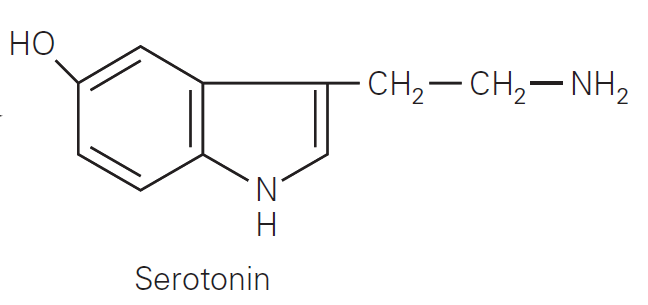
\includegraphics[width=0.6\textwidth]{pictures/Bilder_monoamine_systeme/serotonin.PNG}
    \caption[Serotonin]{\textbf{Serotonin.} Abbildung aus \textit{Principles of Neural Systems}, Kandel et al. \textsuperscript{\cite[Kap.~13]{kandel2013principles}}.}
    \label{fig:serotonin}
\end{figure}{}

Die absteigenden serotonergen Fasern entspringen der medianen Zone der Formatio reticularis im Bereich der Medulla. Aufgrund ihrer medianen Lage werden die serotonergen Kernbegiete auch Raphé-Kerne (griechisch: raphé =~Naht) genannt \textsuperscript{\cite[Kap.~6]{trepel2011neuroanatomie}}. Die \textit{Nuclei raphes}\index{Nuclei! raphes} (Abb.~\ref{fig:raphe_nuclei}) bestehen aus mehreren Teilbeieten, zu denen unter anderem der Nucleus raphé magnus, obscurus und pallidus gehören \textsuperscript{\cite[Kap.~15]{paxinos2014rat}}. Die weitreichenden Projektionen dieser Kerngebiete sind weit im Hirnstamm verteilt. Sie enden unter anderem im Thalamus, Hypothalamus, Striatum, Hippocampus, Cerebellum, Rückenmark, in der Amygdala und in Bereichen des cerebralen Cortex \textsuperscript{\cite[Kap.~9]{crossman2014neuroanatomy}}. 

\begin{figure}[H]
    \centering
    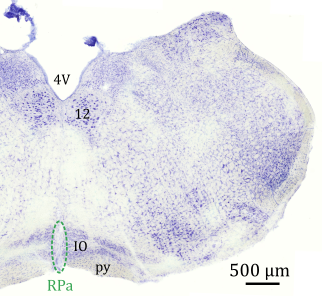
\includegraphics[width=0.5\textwidth]{pictures/Bilder_monoamine_systeme/raphe_nuclei.png}
    \caption[Raphé-Kerne]{\textbf{Raphé-Kerne} (N03-1). Die Raphé-Kerne sind in der Medulla lokalisiert. Zu sehen ist der Nucleus raphé pallidus (\textbf{RPa}), sowie die inferiore Olive (\textbf{IO}), der Pyramidentrakt (\textbf{py}), das Kerngebiet der Nervus hypoglossus (\textbf{12}), sowie der vierte Ventrikel (\textbf{4V}).}
    \label{fig:raphe_nuclei}
\end{figure}

Die Projektionen in den cerebralen Cortex sind in kognitive Funktionen, sowie in die neuronalen Mechanismen von Schlaf und  Gemütszuständen involviert. Ausgehend vom \textit{Nucleus raphé magnus} verlaufen Projektionen ins Rückenmark. Diese sind an der Modulation nozirezeptiver Mechanismen beteiligt \textsuperscript{\cite[Kap.~9]{crossman2014neuroanatomy}}. Durch die Projektionen ins limbische System beeinflusst das serotonerge System zudem emotionale Vorgänge. Einige der serotonergen Bahnen enden in der Formatio reticularis. Dadurch sind die serotonergen Neurone der Raphé-Kerne, wie auch die noradrenergen Neurone des Locus coeruleus, funktionell am Schlaf-Wach-Rhythmus beteiligt \textsuperscript{\cite[Kap.~6]{trepel2011neuroanatomie}}. Auch in die Regulation von Aufmerksamkeit, sowie anderen komplexen kognitiven Funktionen, ist das serotonerge System involviert \textsuperscript{\cite[Kap.~46]{kandel2013principles}}. Ähnlich wie die noradrenergen sind die serotonergen Neurone an der Entstehung von Depressionen, sowie von Angst- und Panikkrankheiten beteiligt. Auch bei der Entstehung von Migräne spielen sie eine wichtige Rolle \textsuperscript{\cite[Kap.~6]{trepel2011neuroanatomie}}.

\begin{figure}[H]
    \centering
    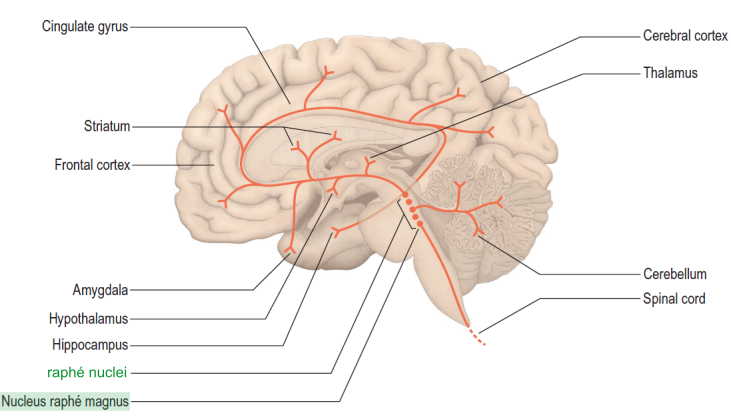
\includegraphics[width=\textwidth]{pictures/Bilder_monoamine_systeme/serotonerges_system.PNG}
    \caption[Serotonerges System]{\textbf{Serotonerges System.} Die serotonergen Neurone sind in den Raphé-Kernen lokalisiert. Diese liegen medial im Teil der Formatio reticularis, der zur Medulla gehört. Abbildung nach \textit{Neuroanatomy}, Crossman und Neary \textsuperscript{\cite[Kap.~9]{crossman2014neuroanatomy}}.}
    \label{fig:serotonerges_system}
\end{figure}{}

